\documentclass[tikz,border=8pt]{standalone}
\usepackage{fontspec}
\setsansfont{Arial}
\usetikzlibrary{arrows.meta,positioning,fit}
% T41 study flow. Source: docs/t41-results.md and docs/t41-handoff.md (PR #25).
\begin{document}
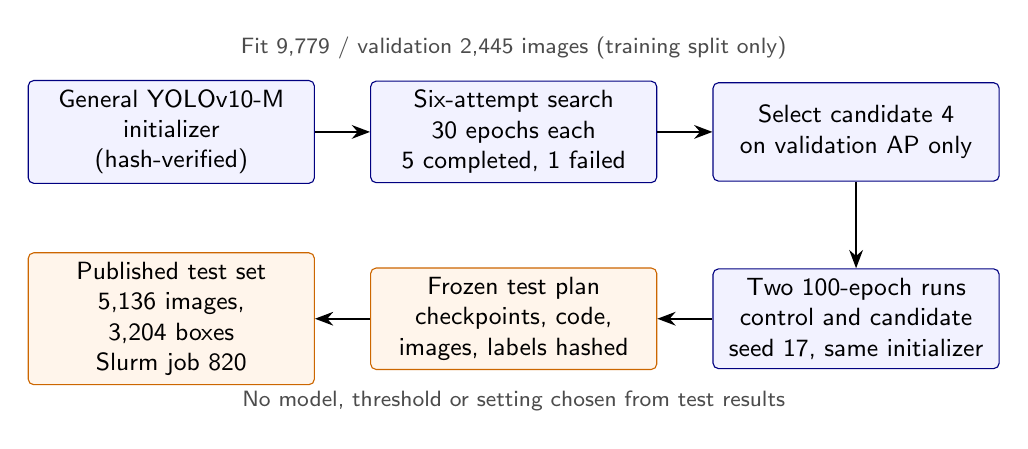
\begin{tikzpicture}[font=\sffamily\small,>=Stealth,
box/.style={draw=blue!50!black,rounded corners=2pt,fill=blue!5,align=center,text width=3.4cm,minimum height=1.25cm},
test/.style={box,draw=orange!80!black,fill=orange!8},
note/.style={font=\sffamily\footnotesize,text=black!70,align=center}]
\node[box] (init) {General YOLOv10-M\\initializer\\(hash-verified)};
\node[box,right=0.7cm of init] (search) {Six-attempt search\\30 epochs each\\5 completed, 1 failed};
\node[box,right=0.7cm of search] (select) {Select candidate 4\\on validation AP only};
\node[box,below=1.1cm of select] (confirm) {Two 100-epoch runs\\control and candidate\\seed 17, same initializer};
\node[test,left=0.7cm of confirm] (freeze) {Frozen test plan\\checkpoints, code,\\images, labels hashed};
\node[test,left=0.7cm of freeze] (test) {Published test set\\5,136 images, 3,204 boxes\\Slurm job 820};
\draw[->,thick] (init)--(search);
\draw[->,thick] (search)--(select);
\draw[->,thick] (select)--(confirm);
\draw[->,thick] (confirm)--(freeze);
\draw[->,thick] (freeze)--(test);
\node[note,above=0.15cm of search] {Fit 9,779 / validation 2,445 images (training split only)};
\node[note,below=0.15cm of freeze] {No model, threshold or setting chosen from test results};
\end{tikzpicture}
\end{document}
